%! Author = Saeid Yazdani
%! Date = 11/17/2023


\section{Challenges in Design and Test}
\label{sec:design-and-test-challenges}

Ever-increasing functional requirements and the demand for the shortest
time-to-market at low production costs creates a challenging environment
for engineers \autocite{Kopp}.

Customers expect the best quality and reliability at a reasonable price.
Recurring cases of failure in a particular brand or model of an airplane,
a car, or a medical device will damage the reputation.
Such incidents will adversely affect sales figures and reputation.
Reliability and safety of electronic systems are mandatory, and a comprehensive
understanding of risk influences must be the basis of design and manufacturing
approaches.

Designers should note that reliability and safety are \emph{not} tightly coupled
and, at least in the electronics industry, are treated
differently \autocite{Evans}.
For example, if a mechanical relay does not switch on command,
this is considered a reliability issue. But if a relay switches at unintended
instances, we will call this a safety issue.
Furthermore:

\begin{itemize}[topsep=8pt,itemsep=4pt,partopsep=4pt, parsep=4pt]
    \item  A module can be a very reliable system that eventually breaks down
    at some point in time.
    Such a system is unsafe if no redundancy can ensure proper operation:
    A module can be made safe by adding redundancy.
    If, due to low reliability, the system runs into shutdown or emergency
    operation repetitively, we do not want to bring such a system into the
    application field.
    \item We require high reliability in safe systems because we do not want
    extended downtimes.
\end{itemize}

Safety and reliability are design tasks and must be forecasted over a product's
total lifecycle.
When designers start to develop a safe and reliable system, they need to be
aware of parameters such as:

\begin{itemize}[topsep=8pt,itemsep=4pt,partopsep=4pt, parsep=4pt]
    \item Reliability of components that are going to be utilized in
    the design (\ac{MTBF}).
    \item Quality of the manufacturing process.
    \item Interconnection reliability (\ac{PCB}, wires, relays,
    connectors, etc.)
    \item Coupling effects from thermal flow, electromagnetic crosstalk, and
    \ac{EMC}.
\end{itemize}

As shown in \autoref{fig:testing-in-product-lifecycle}, a systematic approach to
safety and reliability is based on the tight coupling of design and testing for
all phases of the product lifecycle \autocite{Stroud}:

\begin{itemize}[topsep=8pt,itemsep=4pt,partopsep=4pt, parsep=4pt]
    \item \textbf{\emph{Design Stage:}} Detect and identify \emph{design errors}
    through verification.

    \item \textbf{\emph{Fabrication Stage:}} Find \emph{production defects}
    to prevent the leaking of failing products into the market.

    \item \textbf{\emph{Quality Assurance:}}
    Qualification is necessary to get insight into the expected lifetime, or
    time to first fail (\ac{MTBF}, \ac{MTTF}).
    The final test cannot detect pre-damage or weak behavior of a system, and
    qualification methods are mandatory (as part of the release documents).

    \item \textbf{\emph{Service Stage:}}
    Find \emph{operational faults}, preferably before their occurrence
    (preventive maintenance), to issue repairs and parts replacements promptly.
\end{itemize}

\begin{figure}[htbp]
    \centering
    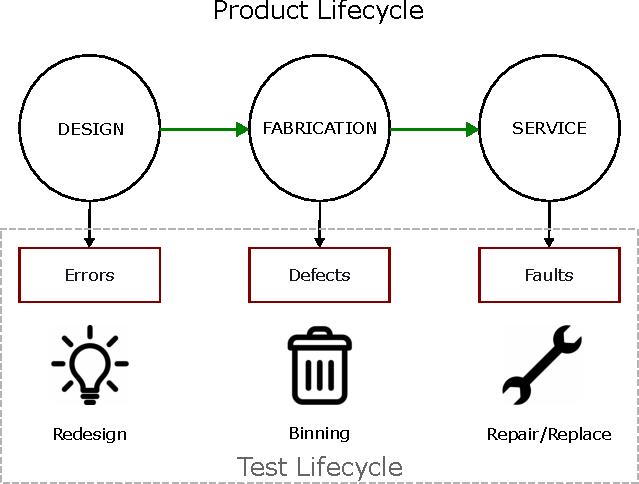
\includegraphics[width=0.86\linewidth,height=0.50\textheight,keepaspectratio]
    {figures/testing-in-product-lifecycle}
    \caption[Product lifecycle and Test are intertwined]{A Typical product
    lifecycle with test lifecycle as a parallel subset.}
    \label{fig:testing-in-product-lifecycle}
\end{figure}

Over the years, a few standards have been developed to limit risk factors.
Thus, all designers must follow standardized design rules and process
flows.
We need a safety certificate for all systems
(UL\footnote{\emph{Underwriters Laboratories}, a global safety science
company headquartered in the USA.} release,
VDE\footnote{\emph{Verband der Elektrotechnik, Elektronik und
Informationstechnik}, a technical-scientific association based in Germany.}
release for electrical, mechanical, chemical and optical safety).
If the function is life-critical (such as airborne systems), we need even more
documents from an independent authority.
Therefore, the whole design process must be quality-oriented.

As stated in \autoref{sec:history-errors-failures-in-electronic-systems},
reliability, safety, and security of electronic systems are of primary interest
in all application areas.
With every crash of an airplane, a power plant, a car, etc., a set of
fundamental questions will arise: Why did it happen, what was not supervised
and what was not thoroughly understood?
As a result, designers of such systems are under pressure to guarantee the
utmost level of reliability and safety.
Strategies for monitoring critical
states must be developed, and we need to get warnings to counteract this.
This again encompasses all phases of product life:

\begin{itemize}[topsep=8pt,itemsep=4pt,partopsep=4pt, parsep=4pt]

    \item Monitor stress influences during the production and transportation
    of safety-critical systems.

    \item Monitor and evaluate stress factors during operation
    (Built-in State Monitors).

\end{itemize}

It should be noted that we cannot guarantee error-free systems, and even under
the premise of utmost confidence, there will be some risk of system crash:
We will never be able to foresee all possible fault conditions even if we got
into all details beforehand (Chernobyl: Unforeseen reactor reaction,
Fukushima: Unforeseen damage to all emergency systems,
Airborne / automotive: Unforeseen software misbehavior in case of unknown
environmental conditions, Medical: Same problem with unforeseen
user mistakes and the list goes on...).

There will always be a chance for surprisingly unexpected issues, such as human
errors and physical failures due to external events that were not part of the
fault list in the beginning.
